\documentclass[12pt]{article}
\usepackage[left=1cm, right=1cm, top=2cm,bottom=1.5cm]{geometry} 

\usepackage[parfill]{parskip}
\usepackage[utf8]{inputenc}
\usepackage[T2A]{fontenc}
\usepackage[russian]{babel}
\usepackage{enumitem}
\usepackage[normalem]{ulem}
\usepackage{amsfonts, amsmath, amsthm, amssymb, mathtools,xcolor,accents}
\usepackage{blkarray}

\usepackage{tabularx}
\usepackage{hhline}

\usepackage{accents}
\usepackage{fancyhdr}
\pagestyle{fancy}
\renewcommand{\headrulewidth}{1.5pt}
\renewcommand{\footrulewidth}{1pt}

\usepackage{graphicx}
\usepackage[figurename=Рис.]{caption}
\usepackage{subcaption}
\usepackage{float}

%%Наименование папки откуда забирать изображения
\graphicspath{ {./images/} }

%%Изменение формата для ввода доказательства
\renewcommand{\proofname}{$\square$  \nopunct}
\renewcommand\qedsymbol{$\blacksquare$}

%%Изменение отступа на таблицах
\addto\captionsrussian{%
	\renewcommand{\proofname}{$\square$ \nopunct}%
}
%% Римские цифры
\newcommand{\RN}[1]{%
	\textup{\uppercase\expandafter{\romannumeral#1}}%
}

%% Для удобства записи
\newcommand{\MR}{\mathbb{R}}
\newcommand{\MC}{\mathbb{C}}
\newcommand{\MQ}{\mathbb{Q}}
\newcommand{\MN}{\mathbb{N}}
\newcommand{\MZ}{\mathbb{Z}}
\newcommand{\MTB}{\mathbb{T}}
\newcommand{\MTI}{\mathbb{I}}
\newcommand{\MI}{\mathrm{I}}
\newcommand{\MCI}{\mathcal{I}}
\newcommand{\MCR}{\mathcal{R}}
\newcommand{\MJ}{\mathrm{J}}
\newcommand{\MH}{\mathrm{H}}
\newcommand{\MT}{\mathrm{T}}
\newcommand{\MU}{\mathcal{U}}
\newcommand{\MV}{\mathcal{V}}
\newcommand{\MA}{\mathcal{A}}
\newcommand{\MB}{\mathcal{B}}
\newcommand{\MF}{\mathcal{F}}
\newcommand{\ME}{\mathcal{E}}
\newcommand{\MW}{\mathcal{W}}
\newcommand{\ML}{\mathcal{L}}
\newcommand{\MM}{\mathcal{M}}
\newcommand{\MP}{\mathcal{P}}
\newcommand{\VN}{\varnothing}
\newcommand{\VE}{\varepsilon}
\newcommand{\dx}{\, dx}
\newcommand{\dy}{\, dy}
\newcommand{\dz}{\, dz}
\newcommand{\dd}{\, d}


\theoremstyle{definition}
\newtheorem{defn}{Опр:}
\newtheorem{rem}{Rm:}
\newtheorem{prop}{Утв.}
\newtheorem{exrc}{Упр.}
\newtheorem{problem}{Задача}
\newtheorem{lemma}{Лемма}
\newtheorem{theorem}{Теорема}
\newtheorem{corollary}{Следствие}

\newenvironment{cusdefn}[1]
{\renewcommand\thedefn{#1}\defn}
{\enddefn}

\DeclareRobustCommand{\divby}{%
	\mathrel{\text{\vbox{\baselineskip.65ex\lineskiplimit0pt\hbox{.}\hbox{.}\hbox{.}}}}%
}
\DeclareRobustCommand{\ndivby}{\mkern-1mu\not\mathrel{\mkern4.5mu\divby}\mkern1mu}


%Короткий минус
\DeclareMathSymbol{\SMN}{\mathbin}{AMSa}{"39}
%Длинная шапка
\newcommand{\overbar}[1]{\mkern 1.5mu\overline{\mkern-1.5mu#1\mkern-1.5mu}\mkern 1.5mu}
%Функция знака
\DeclareMathOperator{\sgn}{sgn}

%Функция ранга
\DeclareMathOperator{\rk}{\text{rk}}
\DeclareMathOperator{\diam}{\text{diam}}


%Обозначение константы
\DeclareMathOperator{\const}{\text{const}}

\DeclareMathOperator{\codim}{\text{codim}}

\DeclareMathOperator*{\dsum}{\displaystyle\sum}
\newcommand{\ddsum}[2]{\displaystyle\sum\limits_{#1}^{#2}}
\newcommand{\ddssum}[2]{\displaystyle\smashoperator{\sum\limits_{#1}^{#2}}}
\newcommand{\ddlsum}[2]{\displaystyle\smashoperator[l]{\sum\limits_{#1}^{#2}}}
\newcommand{\ddrsum}[2]{\displaystyle\smashoperator[r]{\sum\limits_{#1}^{#2}}}

%Интеграл в большом формате
\DeclareMathOperator{\dint}{\displaystyle\int}
\newcommand{\ddint}[2]{\displaystyle\int\limits_{#1}^{#2}}
\newcommand{\ssum}[1]{\displaystyle \sum\limits_{n=1}^{\infty}{#1}_n}

\newcommand{\smallerrel}[1]{\mathrel{\mathpalette\smallerrelaux{#1}}}
\newcommand{\smallerrelaux}[2]{\raisebox{.1ex}{\scalebox{.75}{$#1#2$}}}

\newcommand{\smallin}{\smallerrel{\in}}
\newcommand{\smallnotin}{\smallerrel{\notin}}

\newcommand*{\medcap}{\mathbin{\scalebox{1.25}{\ensuremath{\cap}}}}%
\newcommand*{\medcup}{\mathbin{\scalebox{1.25}{\ensuremath{\cup}}}}%

\makeatletter
\newcommand{\vast}{\bBigg@{3.5}}
\newcommand{\Vast}{\bBigg@{5}}
\makeatother

%Промежуточное значение для sup\inf, поскольку они имеют разную высоту
\newcommand{\newsup}{\mathop{\smash{\mathrm{sup}}}}
\newcommand{\newinf}{\mathop{\mathrm{inf}\vphantom{\mathrm{sup}}}}

%Скалярное произведение
\newcommand{\inner}[2]{\left\langle #1, #2 \right\rangle }
\newcommand{\linsp}[1]{\left\langle #1 \right\rangle }
\newcommand{\linmer}[2]{\left\langle #1 \vert #2\right\rangle }

%Подпись символов снизу
\newcommand{\ubar}[1]{\underaccent{\bar}{#1}}

%%Шапка для букв сверху
\newcommand{\wte}[1]{\widetilde{#1}}
\newcommand{\wht}[1]{\widehat{#1}}
\newcommand{\ovl}[1]{\overline{#1}}


%%Трансформация Фурье
\newcommand{\fourt}[1]{\mathcal{F}\left(#1\right)}
\newcommand{\ifourt}[1]{\mathcal{F}^{-1}\left(#1\right)}

%%Символ вектора
\newcommand{\vecm}[1]{\overrightarrow{#1\,}}

%%Пространстов матриц
\newcommand{\matsq}[1]{\operatorname{Mat}_{#1}}
\newcommand{\mat}[2]{\operatorname{Mat}_{#1, #2}}

%Оператор для действ и мнимых чисел
\DeclareMathOperator{\IM}{\operatorname{Im}}
\DeclareMathOperator{\RE}{\operatorname{Re}}
\DeclareMathOperator{\li}{\operatorname{li}}
\DeclareMathOperator{\GL}{\operatorname{GL}}
\DeclareMathOperator{\SL}{\operatorname{SL}}
\DeclareMathOperator{\Char}{\operatorname{char}}
\DeclareMathOperator\Arg{Arg}
\DeclareMathOperator\ord{ord}

%Оператор для образа
\DeclareMathOperator{\Ima}{Im}

%Делимость чисел
\newcommand{\modn}[3]{#1 \equiv #2 \; (\bmod \; #3)}
\newcommand{\nmodn}[3]{#1 \not\equiv #2 \; (\bmod \; #3)}

%%Взятие в скобки, модули и норму
\newcommand{\parfit}[1]{\left( #1 \right)}
\newcommand{\modfit}[1]{\left| #1 \right|}
\newcommand{\sqparfit}[1]{\left\{ #1 \right\}}
\newcommand{\normfit}[1]{\left\| #1 \right\|}

%%Функция для обозначения равномерной сходимости по множеству
\newcommand{\uconv}[1]{\overset{#1}{\rightrightarrows}}
\newcommand{\uconvm}[2]{\overset{#1}{\underset{#2}{\rightrightarrows}}}

%% Функция для добавления круга сверху множества
\newcommand{\Circ}[1]{\accentset{\circ}{#1}}

%% Жирное подчеркивание
\newcommand{\buline}[1]{\textbf{\uline{#1}}}

%%Функция для обозначения нижнего и верхнего интегралов
\def\upint{\mathchoice%
	{\mkern13mu\overline{\vphantom{\intop}\mkern7mu}\mkern-20mu}%
	{\mkern7mu\overline{\vphantom{\intop}\mkern7mu}\mkern-14mu}%
	{\mkern7mu\overline{\vphantom{\intop}\mkern7mu}\mkern-14mu}%
	{\mkern7mu\overline{\vphantom{\intop}\mkern7mu}\mkern-14mu}%
	\int}
\def\lowint{\mkern3mu\underline{\vphantom{\intop}\mkern7mu}\mkern-10mu\int}

%%След матрицы
\DeclareMathOperator*{\tr}{tr}

\DeclareMathOperator*{\symdif}{\bigtriangleup}

% Верхние\нижние пределы
\DeclareMathOperator*\lowlim{\underline{lim}}
\DeclareMathOperator*\uplim{\overline{lim}}

\makeatletter
\renewcommand*\env@matrix[1][*\c@MaxMatrixCols c]{%
	\hskip -\arraycolsep
	\let\@ifnextchar\new@ifnextchar
	\array{#1}}
\makeatother


%% Переопределение функции хи, чтобы выглядела более приятно
\makeatletter
\@ifdefinable\@latex@chi{\let\@latex@chi\chi}
\renewcommand*\chi{{\@latex@chi\smash[t]{\mathstrut}}} % want only bottom half of \mathstrut
\makeatletter

\setcounter{MaxMatrixCols}{20}


\begin{document}
\lhead{Действительный анализ}
\chead{Дьяченко М.И.}
\rhead{Лекция - 8}

\section*{Интеграл Лебега для простых функций}

Пусть $(X,\MM,\mu)$ - измеримое пространство.
\begin{defn}
	Пусть функция $f \colon X \to \MR$, тогда она называется \uwave{простой} в том и только в том случае, когда она измерима, принимает только конечное число значений и любое ненулевое значение принимается на множестве конечной меры. Формально это будет так:
	$$
		f(x) = \ddsum{l = 1}{r} a_l{\cdot}\chi_{F_l}(x), \quad \forall l, \, F_l \in \MM, \quad \forall l_1 \neq l_2 \Rightarrow F_{l_1} \cap F_{l_2} = \VN, \quad \forall l, \, a_l \neq 0 \Rightarrow \mu(F_l) < \infty
	$$
\end{defn}
\begin{rem}
	Ненулевые значения на множестве конечной меры необходимы только если у нас $X$ $\sigma$-конечно. Для конечного измеримого пространства и так понятно, что ненулевые значения будут на множестве конечной меры. Также заметим, что по нашему определению, простая функция автоматически является измеримой.
\end{rem}

\begin{rem}
	Если $f(x)$ - простая, то её можно представить в виде: 
	$$
		f(x) = \ddsum{k = 1}{n}c_k{\cdot}\chi_{E_k}(x)
	$$
	где $c_1 < c_2 < \dotsc < c_n, \, \forall k, \, E_k \in \MM$ и $\bigsqcup\limits_{k = 1}^{n} E_k = X$, причем если $c_k \neq 0$, то $\mu(E_k) < \infty$.
\end{rem}

\begin{defn}
	Пусть $f(x)$ это простая функция, тогда \uwave{интегралом Лебега} называется сумма вида:
	$$
		\ddint{X}{}f(x)d\mu = \ddsum{l = 1}{r}a_l{\cdot}\mu(F_l)
	$$
	где формально считаем, что: $0{\cdot}\infty= 0$ (поскольку мера у нас $\sigma$-конечна).
\end{defn}

\begin{rem}
	В тех местах, где нам потребуется различать интегралы Римана и интегралы Лебега, мы будем обозначать интеграл Лебега через $(\ML)$:
	$$
		(\ML) \ddint{X}{}f(x)d\mu = \ddint{X}{}f(x)d\mu
	$$
\end{rem}

Попробуем понять в чем разность между интегралом Римана и интегралом Лебега.

\textbf{Пример}: Пусть у нас есть функция, которая принимает конечное число значений на отрезке $[0,1]$.
\begin{figure}[H]
	\centering
	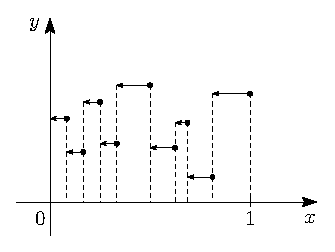
\includegraphics[width=0.35\textwidth]{RAL8_1.eps}
	\caption{Функция принимающая конечное число значений.}
	\label{8_1}
\end{figure}
Тогда по построениею интегралов:
\begin{enumerate}[label = \arabic*)]
	\item \buline{Интеграл Римана}: Надо разбить отрезок $[0,1]$ на отдельные интервалы фиксированной длины, берём значение функции на этом интервале, умножаем и так для каждого интервала. Затем мы уменьшаем длину каждого интервала;
	\item  \buline{Интеграл Лебега}: Надо посмотреть значения на оси $y$, а затем посмотрим какова мера прообразов этих значений. В нашем случае - суммарная длина интервалов на которых функция принимает конкретные значения. Затем мы значения умножаем на меру интервала и складываем;
\end{enumerate}

\begin{prop}
	Определение интеграла Лебега для простых функций корректно, то есть не зависит от способа представления функции.
\end{prop}
\begin{proof}
	Пусть $f(x)$ - простая и имеются представления:
	$$
		f(x) = \ddsum{l = 1}{r}a_l{\cdot}\chi_{F_l}(x) = \ddsum{k = 1}{n}c_k{\cdot}\chi_{E_k}(x)
	$$
	где все $F_l, \, E_k$ - измеримые множества, $c_1 < c_2 < \dotsc < c_n$, $\bigsqcup\limits_{l = 1}^{r}F_l = \bigsqcup\limits_{k = 1}^{n}E_l= X$ и ненулевые значения принимаются на множествах конечной меры. Заметим, что тогда:
	$$
		\forall a_l, \, \exists \, c_k \colon a_l = c_k
	$$
	поскольку значения складываться не могут и каждое принимается на своём множестве. Обозначим:
	$$
		\Gamma_k = \{l \in \{1,2,\dotsc,r\} \colon a_l = c_k\} \Rightarrow \bigsqcup\limits_{l \in \Gamma_k}F_l = E_k \wedge \bigsqcup\limits_{k = 1}^{n}\Gamma_k = \{1,2,\dotsc,r\}
	$$
	где последнее верно в силу того, что все $c_k$ у нас разные $\Rightarrow \Gamma_k$ не могут пересекаться между собой. Следовательно, рассмотрим следующую сумму:
	$$
		\ddsum{k = 1}{n}c_k{\cdot}\mu(E_k) = \ddsum{k = 1}{n}c_k\ddsum{l \in \Gamma_k}{}\mu(F_l) = \ddsum{k = 1}{n}\ddsum{l \in \Gamma_k}{}a_l{\cdot}\mu(F_l) = \ddsum{l = 1}{r}a_l{\cdot}\mu(F_l)
	$$
\end{proof}

\begin{theorem} (\textbf{Линейность интеграла Лебега})
	Пусть $f(x)$ и $g(x)$ - простые и $\alpha,\beta \in \MR^1$, тогда линейная комбинация этих функций: $\alpha{\cdot}f(x) + \beta{\cdot}g(x)$ тоже простая функция и будет верно:
	$$
		\ddint{X}{}\left(\alpha{\cdot}f(x) + \beta{\cdot}g(x) \right) d\mu = \alpha{\cdot}\ddint{X}{}f(x)d\mu + \beta {\cdot}\ddint{X}{}g(x)d\mu
	$$
\end{theorem}
\begin{proof}
	Пусть: $f(x) = \sum\limits_{k = 1}^{n}c_k{\cdot}\chi_{E_k}(x)$ и $g(x) = \sum\limits_{j = 1}^{m}d_j{\cdot}\chi_{S_j}(x)$, где $E_k, \, S_j \in \MM$, $\bigsqcup\limits_{k = 1}^{n}E_k = \bigsqcup\limits_{j = 1}^{m}S_j = X$ и любое ненулевое значение принимается на множестве конечной меры. Тогда:
	$$
		\alpha{\cdot}f(x) + \beta{\cdot}g(x) = \ddsum{k = 1}{n}\ddsum{j = 1}{m}(\alpha{\cdot}c_k + \beta{\cdot}d_j){\cdot}\chi_{E_k \cap S_j}(x)
	$$
	Видно, что эта функция принимает конечное число значений (не больше, чем $n{\cdot}m$), каждое значение принимается на некотором измеримом множестве, кроме того нетрудно заметить:
	$$
		\bigsqcup\limits_{k = 1}^{n}\bigsqcup\limits_{j = 1}^{m}E_k \cap S_j = X
	$$
	Также заметим, что если $\alpha{\cdot}f(x) + \beta{\cdot}g(x) \neq 0$, то хотя бы одно из значений $c_k$ или $d_j$ не должны быть равны нулю $\Rightarrow$ должна быть конечная мера у $E_k$ или $S_j \Rightarrow$ конечная мера у пересечения. Следовательно, функция: $\alpha{\cdot}f(x) + \beta{\cdot}g(x)$ - простая. В силу того, что определение интеграла корректно, то:
	$$
		\ddint{X}{}\left(\alpha{\cdot}f(x) + \beta{\cdot}g(x) \right) d\mu = \ddsum{k = 1}{n}\ddsum{j = 1}{m}(\alpha{\cdot}c_k + \beta{\cdot}d_j){\cdot}\mu(E_k \cap S_j) = \alpha \ddsum{k = 1}{n}c_k\ddsum{j = 1}{m}\mu(E_k \cap S_j) + 
	$$
	$$
		+ \beta\ddsum{j = 1}{m}d_j\ddsum{k = 1}{n}\mu(E_k \cap S_j) = \alpha \ddsum{k = 1}{n}c_k\mu(E_k ) + \beta \ddsum{j = 1}{m}d_j\mu(S_j) = \alpha{\cdot}\ddint{X}{}f(x)d\mu + \beta {\cdot}\ddint{X}{}g(x)d\mu
	$$
\end{proof}

\begin{prop}
	Если $f(x)$ простая и $f(x) \geq 0$, то $\int\limits_{X}f(x)dx \geq 0$.
\end{prop}
\begin{proof}
	Вытекает сразу из определения простой функции и интеграла Лебега:
	$$
		f(x) =  \sum\limits_{k = 1}^{n}a_k{\cdot}\chi_{F_k}(x) \geq 0 \wedge \forall k, \, \mu(F_k) \geq 0 \Rightarrow \ddint{X}{}f(x)d\mu = \ddsum{k = 1}{n}a_k{\cdot}\mu(F_k) \geq 0
	$$
\end{proof}
\begin{prop}
	Если $f(x)$ и $g(x)$ - простые и $\forall x \in X, \, f(x) \geq g(x)$, то будет верно:
	$$
		\ddint{X}{}f(x)d\mu \geq \ddint{X}{}g(x) d\mu
	$$
\end{prop}
\begin{proof}
	Сразу следует из предыдущего утверждения и линейности интеграла:
	$$
		\forall x \in X, \, f(x) \geq g(x) \Rightarrow f(x) - g(x) \geq 0 \Rightarrow \ddint{X}{}(f(x) - g(x))d\mu = \ddint{X}{}f(x) d\mu - \ddint{X}{}g(x) d\mu \geq 0
	$$
\end{proof}
\begin{prop}
	Если $f(x)$ - простая, то и $|f(x)|$ - тоже простая функция, кроме того:
	$$
		\left|\ddint{X}{}f(x)d\mu\right| \leq \ddint{X}{}|f(x)|d\mu
	$$
\end{prop}
\begin{proof}
	Исходная функция принимала не более конечного числа значений $\Rightarrow |f(x)|$ число значений может лишь уменьшиться. Кроме того верно:
	$$
		\left| \ddsum{k = 1}{n}c_k {\cdot}\mu(E_k)\right| \leq \ddsum{k = 1}{n}|c_k|{\cdot}\mu(E_k) 
	$$
\end{proof}

\begin{prop}
	Если $\mu(X) < \infty$, то $f(x) \equiv c$ это простая функция. Тогда:
	$$
		\ddint{X}{}f(x)d\mu = c{\cdot}\mu(X)
	$$
\end{prop}
\begin{proof}
	Так как $\mu(X) < \infty$ и функция $f(x)$ принимает лишь одно значение на всём $X \Rightarrow$ она простая. Тогда:
	$$
		\ddint{X}{}f(x)d\mu = \ddsum{k = 1}{n}c{\cdot}\mu(E_k) = c{\cdot}\ddsum{k = 1}{n}\mu(E_k)= c{\cdot}\mu\left(\bigsqcup\limits_{k = 1}^{n}E_k\right) = c{\cdot}\mu(X)
	$$
\end{proof}

\begin{defn}
	Пусть $\{f_n(x)\}_{n = 1}^{\infty}$ - последовательность функций на $X$, тогда скажем, что она \uwave{монотонно не убывает} на $X$ в том и только в том случае, когда:
	$$
		\forall x \in X,\, \forall n \in \MN, \, f_{n+1}(x) \geq f_n(x)
	$$
	\buline{Обозначение}: $f_n(x) \uparrow$ или $f_n(x) \uparrow f(x)$ если известно к чему она сходится.
\end{defn}

\begin{theorem}
	Пусть $\{g_n(x)\}_{n = 1}^{\infty}$, где $g_n(x)$ это простые неотрицательные функции на $X$, $g_n(x) \uparrow$ на $X$ и кроме того:
	$$
		\forall x \in X, \, g(x) \leq \lim\limits_{n\to \infty}g_n(x) 
	$$
	Тогда будет верно неравенство:
	$$
		\ddint{X}{}g(x) d\mu \leq \lim\limits_{n \to \infty} \ddint{X}{}g_n(x)d\mu
	$$	
	где справа возможно значение $\infty$.
\end{theorem}
\begin{proof}
	Пусть $g(x) = \sum\limits_{r = 1}^{s} a_r{\cdot}\chi_{E_r}(x)$, где $E_r \in \MM, \, E_{r_1} \cap E_{r_2} = \VN$ при $r_1 \neq r_2$ и $0 < a_1 < \dotsc < a_s$. Обозначим:
	$$
		F = \bigsqcup\limits_{r = 1}^{s}E_r \Rightarrow \mu(F) < \infty
	$$
	где последнее верно в силу того, что все значения $a_i$ ненулевые (даже если у нас $\sigma$-конечное пространство). Тогда $\forall \VE > 0$ и для $\forall n$ определим множество:
	$$
		F_n(\VE) = \{x \in F \colon g_n(x) < g(x) - \VE\}
	$$
	Так как $g_n(x) \uparrow$, то мы имеем: $F \supseteq F_1(x) \supseteq F_2 \supseteq \dotsc $, при этом, поскольку: $\lim\limits_{n \to \infty}g_n(x) \geq g(x)$, то:
	$$
		\bigcap\limits_{n = 1}^{\infty}F_n(\VE) = \VN
	$$
	Следовательно, по теореме о непрерывности меры (в силу $\mu(F) < \infty$), мы получим:
	$$
		\mu(F_n(\VE)) \xrightarrow[n\to \infty]{} 0	
	$$
	Заметим, что если: $X = A \sqcup B$, причём $A,B \in \MM$ и $h(x)$ это простая функция на $X$, то $h(x)$ простая и на $A$, и на $B$. В результате:
	$$
		h(x) = h(x){\cdot}\chi_A(x) + h(x){\cdot}\chi_B(x) \Rightarrow 
	$$
	$$
		\Rightarrow \ddint{X}{}h(x)d\mu = \ddint{X}{}h(x){\cdot}\chi_A(x) d\mu + \ddint{X}{}h(x){\cdot}\chi_B(x) d \mu = \ddint{A}{}h(x) d\mu + \ddint{B}{}h(x) d\mu
	$$
	В конечном счёте, поскольку $g(x) \leq a_s$, где $a_s$ - максимальное значение для $g(x)$, то тогда для любого $n$ будет верно:
	$$
		\ddint{X}{}g(x)d\mu = \ddint{F}{}g(x)d\mu = \ddint{F_n(\VE)}{}g(x) d\mu + \ddint{F \setminus F_n(\VE)}{}g(x)d\mu \leq \ddint{F_n(\VE)}{}a_sd\mu + \ddint{F \setminus F_n(\VE)}{}(g_n(x) + \VE)d\mu \Rightarrow
	$$
	$$
		\Rightarrow \ddint{X}{}g(x)d\mu \leq a_s{\cdot}\mu(F_n(\VE)) + \ddint{X}{}g_n(x)d\mu -\ddint{X \setminus (F \setminus F_n(\VE))}{}g_n(x) d\mu + \VE {\cdot}\mu(F\setminus F_n(\VE)) \leq 
	$$
	$$
		\leq a_s{\cdot}\mu(F_n(\VE)) + \VE{\cdot}\mu(F) + \ddint{X}{}g_n(x)d\mu \Rightarrow a_s{\cdot}\mu(F_n(\VE)) \xrightarrow[n \to \infty]{} 0 \Rightarrow \ddint{X}{}g(x)d\mu  \leq \lim\limits_{n \to \infty}\ddint{X}{}g_n(x)d\mu + \VE{\cdot}\mu(F)
	$$
	Поскольку $\VE > 0$ - произвольное, то мы получаем утверждение теоремы.
\end{proof}

\newpage
\section*{Интеграл Лебега}

Пусть $(X, \MM,\mu)$ это измеримое пространство.

\begin{defn}
	Пусть $f(x)$ измерима и неотрицательна на $X$, тогда \uwave{множеством минорантных функций} для неё называется множество неотрицательных простых функций: 
	$$
		Q_f = \{\text{простые функции } \varphi(x) \colon 0 \leq \varphi(x) \leq f(x), \, \forall x \in X\}
	$$
\end{defn}

\begin{rem}
	Всегда функция $0 \in Q_f$ и следовательно: $Q_f  \neq \VN$.
\end{rem}

\begin{defn}
	Пусть $f(x)$ измерима и неотрицательна на $X$, тогда \uwave{интегралом Лебега} функции $f(x)$ по множеству $X$ называется точная верхняя грань:
	$$
		(\ML) \ddint{X}{}f(x)d\mu = \ddint{X}{}f(x) d\mu = \sup\limits_{\varphi \in Q_f} \ddint{X}{}\varphi(x) d\mu
	$$
	При этом будем говорить, что $f(x) \in \ML(X)$ (\uwave{интегрируема по Лебегу на $X$}) тогда и только тогда, когда интеграл конечен, то есть:
	$$
		f(x) \in \ML(X) \Leftrightarrow \ddint{X}{}f(x)d\mu < \infty
	$$
\end{defn}

Если функция $f(x)$ измерима на $X$, то определим функции:
\begin{enumerate}[label=\arabic*)]
	\item $f_{+}(x) = \max\{f(x), 0\}$;
	\item $f_{-}(x) = - \min\{f(x),0\}$;
\end{enumerate}
Обе функции измеримые и неотрицательные. Заметим, что всегда будет верно равенство:
$$
	\forall x \in X, \, f(x) = f_{+}(x) - f_{-}(x)
$$
\begin{defn}
	Пусть $f(x)$ измерима на $X$, тогда скажем, что $f(x)$ \uwave{интегрируема по Лебегу на $X$}, если интегрируемы функции: $f_{+}(x)$ и $f_{-}(x)$, то есть: 
	$$
		f(x) \in \ML(X) \Leftrightarrow f_{+}(x) \in \ML(X) \wedge f_{-}(x) \in \ML(X)
	$$
	Если это выполнено, то полагаем, что верно равенство:
	$$
		(\ML) \ddint{X}{}f(x)d\mu  = \ddint{X}{}f(x)d\mu = \ddint{X}{}f_{+}(x) d\mu - \ddint{X}{}f_{-}(x)d\mu
	$$
\end{defn}
\begin{rem}
	Есть разные способы ввдеения интеграла Лебега, в данном конкретном случае будет проще доказывать теоремы о предельном переходе, но будет сложнее доказывать теоремы о линейности интеграла Лебега по функции в общей ситуации.
\end{rem}

\newpage
\begin{prop}
	Для простых функций определения $5$ и $6$ дают то же значение интеграла, что и определение $2$.
\end{prop}
\begin{proof}
	В силу определения $6$, если функция простая, то мы её должны разбить на две простые функции, обе из которых будут неотрицательными $\Rightarrow$ достаточно доказать утверждение для простой и неотрицательной функции $f(x)$. Заметим, что сама $f(x) \in Q_f$, поскольку она простая, тогда:
	$$ 
		\sup\limits_{\varphi \in Q_f}\ddint{X}{}\varphi(x)d\mu \geq \ddint{X}{}f(x) d\mu
	$$
	в смысле определения $2$, поскольку среди всех функций в $Q_f$ есть и $f$. С другой стороны, если $\varphi(x) \in Q_f$, то (в смысле определения $2$):
	$$
		\ddint{X}{}\varphi(x)d \mu \leq \ddint{X}{}f(x) d\mu \Rightarrow \sup\limits_{\varphi \in Q_f}\ddint{X}{}\varphi(x)d\mu \leq \ddint{X}{}f(x) d\mu \Rightarrow \sup\limits_{\varphi \in Q_f}\ddint{X}{}\varphi(x)d\mu = \ddint{X}{}f(x) d\mu
	$$
\end{proof}

\begin{prop}
	Пусть $f(x)$ измерима и неотрицательна на $X$, $\{f_n(x)\}_{n = 1}^{\infty}$ - простые неотрицательные функции на $X$ и кроме того $f_n(x) \uparrow f(x)$ на $X$, тогда:
	$$
		\ddint{X}{}f(x)d\mu = \lim\limits_{n \to \infty} \ddint{X}{}f_n(x)d\mu
	$$
\end{prop}
\begin{proof}\hfill
	\begin{enumerate}[label=\arabic*)]
		\item По условию: $\forall n, \, f_n(x) \in Q_f$, поскольку: $\forall n, \, f_n(x) \leq f(x)$, тогда мы получим неравенство:
		$$
			\forall n, \, \ddint{X}{}f(x)d\mu \geq \ddint{X}{}f_n(x)d\mu \Rightarrow \ddint{X}{}f(x)d\mu \geq \lim\limits_{n \to \infty}\ddint{X}{}f_n(x)d\mu 
		$$
		\item Предположим, что некоторая функция $\varphi(x) \in Q_f$, тогда по условию:
		$$
			\lim\limits_{n \to \infty}f_n(x) = f(x) \geq \varphi(x)
		$$
		По теореме $2$ тогда будет верно следующее:
		$$
			\lim\limits_{n \to \infty}\ddint{X}{}f_n(x)d\mu \geq \ddint{X}{}\varphi(x) d\mu \Rightarrow  \lim\limits_{n \to \infty}\ddint{X}{}f_n(x)d\mu \geq \sup\limits_{\varphi \in Q_f}\ddint{X}{}\varphi(x) d\mu = \ddint{X}{}f(x)d\mu
		$$
	\end{enumerate}
\end{proof}

\subsection*{Лемма о сходимости последовательности $f_n(x)$ к $f(x)$}
\begin{lemma}
	Пусть $f(x)$ неотрицательна и измерима на $X$, тогда существует последовательность простых неотрицательных функций: $\{f_n(x)\}_{n = 1}^{\infty}\colon f_n(x) \uparrow f(x)$ на $X$.
\end{lemma}
\begin{proof}
	Пусть $X = \bigsqcup\limits_{j = 1}^{\infty}B_j$, где $\forall j, \, B_j \in \MM, \, \mu(B_j) < \infty$. Если $\mu(X) < \infty$, то полагаем, что: 
	$$
		B_1 = X, \, B_2 = B_3 = \dotsc = \VN
	$$
	Для любого $n$ определим функции $f_n(x)$:
	$$
		f_n(x) = 0{\cdot}\MTI_{X \setminus F_n}(x) + 2^n{\cdot}\MTI_{F_n \cap G_n}(x) + \ddsum{k = 1}{2^{2n}}\dfrac{k - 1}{2^n}{\cdot}\MTI_{F_n \cap H_{k,n}}(x)
	$$
	$$
		F_n = \bigsqcup\limits_{j = 1}^{n}B_j, \quad G_n = \{x \in X \colon f(x) \geq 2^n\}, \quad H_{k,n} = \{x \in X \colon \tfrac{k-1}{2^n} \leq f(x) < \tfrac{k}{2^n}\}, \, \forall k = 1,2,3,\dotsc, 2^{2n}
	$$
	Очевидно, что $f_n(x)$ это простые функции, поскольку принимают конечное число значений $\forall n$ на измеримом множестве (поскольку $F_n$ - измеримы, $G_n$ и $H_{k,n}$ - измеримы для измеримой функции $\Rightarrow$ пересечения тоже измеримы). Проверим, что: $f_n(x) \uparrow$ на $X$:
	\begin{enumerate}[label=\arabic*)]
		\item $\forall n, \, f_n(x) = 0 \Rightarrow f_{n+1}(x) \geq 0 = f_n(x)$;
		\item $\forall n, \, f_n(x) = 2^n \Rightarrow x \in F_n \subseteq F_{n+1} \wedge f(x) \geq 2^n$, тогда: 
		$$
			k = 2^{2n + 1} + 1 \Rightarrow f(x) \geq \dfrac{2^{2n + 1} + 1 - 1}{2^{n+1}} = 2^n \Rightarrow  \dotsc \Rightarrow k = 2^{2n+2} \Rightarrow f(x) \geq 2^{n+1} - \dfrac{1}{2^{n+1}} \Rightarrow
		$$
		$$
			\Rightarrow f_{n+1}(x) \in \{2^n, 2^n + \tfrac{1}{2^{n+1}}, \dotsc, 2^{n+1}\} \Rightarrow f_{n+1}(x) \geq f_n(x)
		$$                                                                    
		\item $\forall  n, \, f_n(x) = \tfrac{k-1}{2^n}, \, k = 1,2,3, \dotsc, 2^{2n} \Rightarrow  x \in F_n \subseteq F_{n+1} \wedge \tfrac{k-1}{2^n} \leq f(x) < \tfrac{k}{2^n}$, тогда:
		$$
			\dfrac{k-1}{2^n} = \dfrac{2k - 2}{2^{n+1}} \leq f(x) < \dfrac{2k}{2^{n+1}} = \dfrac{k}{2^n} \Rightarrow f_{n+1}(x) \in \{\tfrac{2k-2}{2^{n+1}}, \tfrac{2k - 1}{2^{n+1}} \} \Rightarrow f_{n+1}(x) \geq f_n(x)
		$$                                              
	\end{enumerate}	
	Проверим, что: $\forall x \in X, \, f_n(x) \xrightarrow[n \to \infty]{} f(x)$. Если $f(x) < \infty$, то будет верно: 
	$$
		\exists \, n_0 \colon x \in F_{n_0} \wedge f(x) \leq 2^{n_0} \Rightarrow \forall n \geq n_0, \, 0 \leq f(x) - f_n(x) \leq \tfrac{1}{2^n} \Rightarrow f_n(x) \xrightarrow[n \to \infty]{} f(x)
	$$
	Если $f(x) = \infty$, то будет верно:
	$$
		\exists \, n_0 \colon x \in F_{n_0} \Rightarrow \forall n \geq n_0, \, f(x) \geq 2^n \Rightarrow  f_n(x) = 2^n \xrightarrow[n \to \infty]{} \infty
	$$
\end{proof}

\begin{theorem}
	Пусть $f(x)$ и $g(x)$ измеримые и неотрицательные функции на $X$, тогда:
	$$
		\ddint{X}{}(f(x) + g(x))d\mu = \ddint{X}{}f(x) d\mu + \ddint{X}{}g(x) d\mu
	$$
	где мы считаем, что: $\infty + \infty = \infty$ и $\infty + a = \infty$.
\end{theorem}
\begin{proof}
	Согласно лемме $1$ существует последовательность простых неотрицательных функций: $\{f_n(x)\}_{n = 1}^{\infty}$, которые монотонно неубывая сходятся к $f(x) \colon f_n(x) \uparrow f(x)$. Аналогично, $\exists \, \{g_n(x)\}_{n = 1}^{\infty} \colon g_n(x) \uparrow g(x)$. При этом, если мы просуммируем эти последовательности, то: 
	$$
		(f_n(x) + g_n(x)) \uparrow (f(x) + g(x))
	$$
	Согласно утверждению $7$ будет верно:
	$$
		\ddint{X}{}(f(x) + g(x))d\mu = \lim\limits_{n \to \infty}\ddint{X}{}(f_n(x) + g_n(x))d \mu = \lim\limits_{n \to \infty}\ddint{X}{}f_n(x)d\mu + \lim\limits_{n \to \infty}\ddint{X}{}g_n(x) d\mu
	$$
	где последнее верно в силу того, что $f_n(x)$ и $g_n(x)$ - простые. Снова воспользуемся утверждением $7$, тогда:
	$$
		\ddint{X}{}(f(x) + g(x))d\mu = \lim\limits_{n \to \infty}\ddint{X}{}f_n(x)d\mu + \lim\limits_{n \to \infty}\ddint{X}{}g_n(x) d\mu = \ddint{X}{}f(x)d\mu + \ddint{X}{}g(x) d\mu
	$$
\end{proof}
\begin{corollary}
	Если $f(x)$ измерима и неотрицательна на $X$, а $X = A \sqcup B$, где $A, B \in \MM$, то будет верно:
	$$
		\ddint{X}{}f(x)d\mu = \ddint{A}{}f(x)d\mu + \ddint{B}{}f(x)d\mu
	$$
\end{corollary}
\begin{proof}
	Вытекает из равенства: 
	$$
		f(x) = f(x){\cdot}\chi_{A}(x) + f(x){\cdot}\chi_B(x)
	$$
	и того, что согласно определениям $2$ и $5$ будет верно:
	$$
		\ddint{X}{}f(x){\cdot}\chi_A(x)d\mu = \ddint{A}{}f(x)d\mu
	$$
	Подробнее, поскольку $A \subseteq X, \, A \in \MM$, то $f(x) \in \ML(A)$ тогда и только тогда, когда: $f(x)\chi_A(x) \in \ML(X)$ и если $f(x) \in \ML(A)$, то выполнено равенство выше. Очевидно, что это выполнено для простых функций. Пусть $h(x)$ - простая неотрицательная, тогда:
	$$
		\forall x \in A, \, 0 \leq h(x) \leq f(x) \Rightarrow \forall x \in X,\, 0 \leq h(x){\cdot}\chi_A(x) \leq f(x){\cdot}\chi_A(x)
	$$
	Обратно будет верно:
	$$
		\forall x \in X, \, 0 \leq h(x) \leq f(x){\cdot}\chi_A(x) \Rightarrow \forall x \in X \setminus A, \, h(x) = 0 \Rightarrow 
	$$
	$$
		\Rightarrow h(x) = h(x){\cdot}\chi_A(x) \Rightarrow \forall x \in A, \, 0 \leq h(x) \leq f(x)
	$$
	Тогда:
	$$
		\ddint{X}{}f(x){\cdot}\chi_A(x)d\mu = \sup\limits_{h \in Q_f}\ddint{X}{}h(x){\cdot}\chi_A(x)d\mu =\sup\limits_{h \in Q_f}\ddint{A}{}h(x)d\mu = \ddint{A}{}f(x)d\mu
	$$
\end{proof}

\end{document}